\documentclass[b5paper]{article}
% 超链接
\usepackage[colorlinks]{hyperref}
% 插入图片
\usepackage{graphicx}
% 设置中文环境
\usepackage[heading=true, fontset=none, UTF8]{ctex} 
\setCJKmainfont[ItalicFont={KaiTi_GB2312}, BoldFont={SimHei}]{SimSun}
\setCJKsansfont{SimHei}
\setCJKmonofont{FangSong_GB2312}
% 黑体
\setCJKfamilyfont{heiti}{SimHei}             
\newcommand{\heiti}{\CJKfamily{heiti}}
% 楷体 GB2312
\setCJKfamilyfont{kaishu}{KaiTi_GB2312}             
\newcommand{\kaishu}{\CJKfamily{kaishu}}
% 宋体
\setCJKfamilyfont{songti}{SimSun}             
\newcommand{\songti}{\CJKfamily{songti}}
% 仿宋 GB2312
\setCJKfamilyfont{fangsong}{FangSong_GB2312}             
\newcommand{\fangsong}{\CJKfamily{fangsong}}

\usepackage{amsmath,bm} % 处理数学公式

\usepackage{mathpazo} % 数学符号
\usepackage{palatino} % 英文衬线字体
\usepackage{courier}  % 英文无衬线字体
\usepackage[T1]{fontenc} % 字体编码 T1

\usepackage{xcolor}
\definecolor{shadecolor}{rgb}{.97, .97, .97}

\usepackage{listings}
\lstset{
  basicstyle=\ttfamily, % 代码是等宽字体
  backgroundcolor=\color{shadecolor},  % 代码块的背景颜色
  breaklines=true, % 可以段行
  numbers=left,    % 行序号
  numberstyle=\footnotesize, % 行序号字体大小
  commentstyle=\ttfamily     % 注释是等宽字体
}

\title{LaTeX 入门}
\author{张三}
\begin{document}
\maketitle
\tableofcontents
\section{线性模型} \label{sec:lm}
第 \ref{sec:lm} 节是线性模型。
\begin{align} \label{eq:lm}
\bm{\mathsf{y}} = \bm{\mathsf{X}}\bm{\beta} + \bm{\epsilon}
\end{align}
公式 \ref{eq:lm} 是线性模型的矩阵表示。

\[
\Bigg(\sqrt{\frac{M}{1 - \big(\frac{r}{\widetilde{x_1 + \cdots + u_N}} \big)^2} \big(\sum_{\beta =1}^{N} \sum_{i=1}^{n}\frac{\partial u_{\beta}}{\partial x_i} + 1 \big) } + \sqrt{XY} \Bigg)^3
\]

\begin{verbatim}
library(stats) % 提供 lowess, rpois, rnorm 等函数
library(graphics) % 提供 plot 方法
plot(cars)
lines(lowess(cars))
\end{verbatim}

\begin{lstlisting}[language=R]
library(stats)    % 提供 lowess, rpois, rnorm 等函数
library(graphics) % 提供 plot 方法
plot(cars)
lines(lowess(cars))
\end{lstlisting}

表格 \ref{tbl:demo}

\begin{table}[h!]
  \begin{center}
    \begin{tabular}{|c c c|} 
      \hline
      列1 & 列2 & 列3 \\ 
      \hline
      1 & 6 & 77 \\ 
      2 & 7 & 15 \\
      3 & 8 & 44 \\
      \hline
    \end{tabular}
  \caption{表格的标题}
  \label{tbl:demo}
  \end{center}
\end{table}

\begin{figure}[ht]
  \begin{center}
    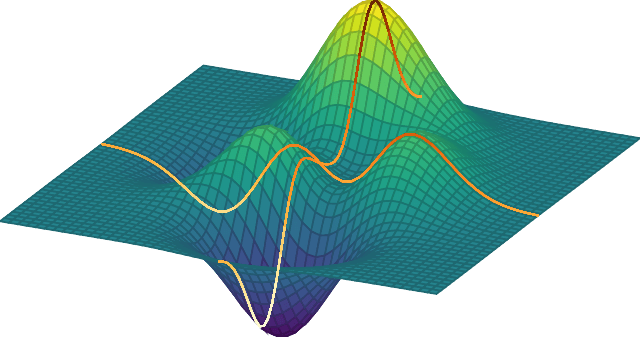
\includegraphics[width=.75\textwidth]{../images/peaks.png}
    \caption{图片的标题}
    \label{fig:figure}
  \end{center}
\end{figure}

\end{document}
